\section{Lessons Learned}
This work makes use of semantic constraint validation to support explainable AI. Semantic constraint validation excels in checking structured data against constraints. Machine learning models in the context of explainable AI are often model-inherent explainable. Nevertheless, their predictions lack rationality for human constraints or scientific facts. Combining explainable AI with semantic constraint validation allows for interpretability and explainability combing with more trust in predictions.

Technically, the concepts were combined by aligning the entities in the knowledge graph (i.e., the set of seed nodes) with the samples in the dataset by the sample-to-node mapping. Two types of constraints are proposed: \emph{Prediction constraints} can be used to explain and check the model's predictions based on a correct data basis. The semantic context of the problem instance (represented through an entity in the knowledge graph) is used to grade the prediction to be correct or incorrect. If the prediction is correct, an explanation is found for the prediction. On the contrary, the constraints' statement reasons why the prediction is wrong and may be used to improve the model. \emph{Data constraints} measure the trustworthiness of the samples in the dataset. They are able to do so since they measure the integrity of the semantic context of the entities to be valid or invalid\footnote{or even not applicable in the case of the 3-valued logic}.

The first problem formulated is the efficient validation of the constraints over the machine learning model given the semantic context of the entities in the dataset. It is tackled by a validation engine integrating the dataset extraction, the model training, the SHACL validation, and the constraint validation. Heuristics are proposed to speed up the execution of the engine, exploiting the actual need for SHACL validation results, the join strategy, caching of intermediate results, and vectorization techniques. A Python implementation for the engine is provided. As well as the approach, the implemented engine is agnostic to the machine learning model and the SHACL engine. Based on the implementation, the approach is evaluated with respect to the engine's performance.
The evaluation is conducted using two synthetic and two non-synthetic benchmarks. Minimizing the number of SHACL validation results by generating only the required SHACL validation results for each constraint at a time and avoiding re-evaluation of shapes, the execution time of the SHACL validation could be reduced to 6\% of a naive approach not using the heuristics. Choosing a good join strategy does impact, but the total time savings are less than the total time savings from optimizing the SHACL validation, as joining is a less complex operation. 

The second problem formulated is the summarization of the knowledge gained through validating the constraints to make the behavior of the machine learning model clearer to the user. Frequency distribution tables are consulted for the summarization of a single constraint. A concept, referred to by coverage, allowed to reduce the constraint validation results of multiple constraints by prioritizing. Based on that, model-coherent summaries are created for decision trees in the form of annotated decision trees. The visualizations created this way are based on the dtreeviz library, but implemented to support the parallel node plot generation and the annotation with the validation results of multiple constraints. The experimental evaluation has shown that the parallelization approach is not yet mature, but the coverage allows visualizing multiple constraints with a less than linear increasing execution time. A comparison of the visualization algorithms' execution time with the execution time of the dtreeviz library showed that it scales considerably better w.r.t. the number of samples in the dataset, but slightly worse w.r.t. the depth of the decision tree visualized. % reason:  vectorization with NumPy and caching of intermediate results

The overall approach is integrated into the InterpretME pipeline, and an evaluation of the pipeline has shown that the methods in this work can provide improved interpretability. Visualization-specific interpretations w.r.t. over- and underfitting are given as a suggestion for further constraint-depending interpretations.

\section{Limitations}
The approach proposed in this work comes with some limitations. 
% The dataset has to be extractable from a knowledge graph --> to apply the heuristics efficiently the seed nodes need to identify in a simple way (maybe materialization is needed)
First, it is assumed that the dataset is extractable from a knowledge graph. Although the semantic web continuously grows, most of the time, the data will not be instantly available as a knowledge graph. In that case, the available (un)structured data needs to be transformed into RDF knowledge graphs (e.g., using mapping rules \cite{rdfizer}). However, the transformation alone will most likely not be enough when the entities in the data do not come with a sufficient semantic context, which goes beyond the features to be extracted for each entity. This implies that the knowledge graph may have to be extended or connected with further data. As turned out in section \ref{section_evaluation_summary}, the heuristics require a simple seed query to be used efficiently. Therefore the set of seed nodes may need to be marked with a class. So in this case it is also necessary to have the SPARQL endpoint either locally available or the permissions for modifications.

% Time complexity-based limitations of the validation engine
Next, extracting the dataset has to be possible in an efficient way (i.e., such that the time to execute the SPARQL query is reasonable), this may require further modifications to the knowledge graph. As the constraints are defined based on SHACL, the constraints can only be as expressive as the SHACL specification allows, given the knowledge graph. Specific constraints involving negations in recursive dependencies may not be evaluated in polynomial time by a SHACL engine (see section \ref{section_validation_engine_complexity}).

% Interpretability is based on domain knowledge
% Scalability of rule-based explanations
Further, as usual for approaches making use of rule-based explanations, domain knowledge is needed to define the constraints as well as to interpret the results. Most likely the constraints need to be user-specified to be well understood. User-defined constraints also come with the short-coming of only detecting patterns in the data, which are also suspected (e.g., one can only detect persons with an invalid birth date, if one creates a constraint that checks for it).

% Explanations can only be valid if the data basis for them is valid
% Statements about the model can only be made with a sufficiently large and diverse data basis --> sample-to-node mapping
Finally, \emph{Data Constraints} can be used to check for the integrity (i.e., trustworthiness) of the data. This is even necessary as explanations are only available for \emph{Prediction Constraints}, which do require a valid data basis to be applicable. Moreover, to check a model \emph{indirectly} against facts encoded as constraints, the data basis has to be large and diverse enough. This is especially an obstacle if a small subset of the available data should be used for validation (see section \ref{section_algorithms_performance_measures}), which will not contain a problem instance for every harmful case one might want to detect. The latter is usually referred to by the \emph{curse of dimensionality} \cite{bishop2006pattern}. 

\section{Future Work}
In future work, the visualization approach may be extended to further machine learning models (i.e., based on decision trees: Random Forests, AdaBoost Gradient Boosting). Figure \ref{fig:random_forest_draft} shows a draft for the visualization of the prediction a random forest makes based on a problem instance. The dtreeviz library is continuously extended, e.g., by adding a visualization of the classification boundaries or the feature-target space. Both kinds of visualizations could be used to further show the constraint validation results in different contexts. Section \ref{section_valSPARQL} presented the theory of performing SHACL constraint validation during the SPARQL query execution and promises further execution time improvements, when applied in a way that avoids the duplicate validation of shapes.

\begin{figure}
    \centering
    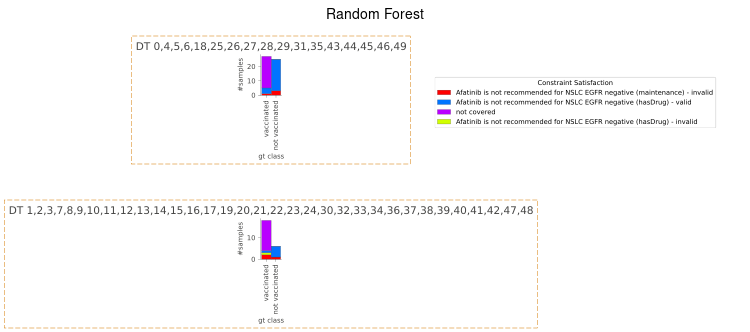
\includegraphics[width=\textwidth]{images/random_forest_exp.png}
    \caption{Draft for the visualization showing the representative leaves in a random forest corresponding to a specific prediction given a problem instance. The bootstrapping process is tracked, to identify the samples on which the prediction is based for each decision tree. Similar constraint validation result distributions are clustered using KMeans and only a representative per cluster is shown. The orange border indicates that the majority of decision trees in the cluster voted for the prediction. \textit{The Lung Cancer KG} provides the data on which the random forest is trained.}
    \label{fig:random_forest_draft}
\end{figure}